\chapter{Methoden und Techniken} \label{cha:Methoden}
    In diesem Kapitel geht es um die grundlegenden Bedingungen zur Untersuchung von Molekülen auf antiferromagnnetischen Oberflächen.
    Dazu gehört zunächst das Ultrahochvakuum, welches notwendig ist um eine saubere und wohl definierte Oberfläche zu erhalten.
    Ferner wird die Methode Beugung niederenergetischer Elektronen erläutert, womit auf die geometrische Struktur der Oberfläche geschlossen werden kann.
    Anschließend geht es um die Photoelektronenspektroskopie und ihre Teilbereiche, welche eine Untersuchung der elektronischen Struktur zuläst.

    \section{Grundlegende Bedingungen} \label{sec:Grundlagen}
        Um sich Oberflächen genauer anzusehen muss zunächst verhindert werden, dass sich keine unerwünschten Teilchen auf der Oberfläche absetzen.
        Hierzu wird Ultrahochvakuum (UHV) eingesetzt.
        Da es keine Pumpe gibt, die direkt vom Atmosphärendruck bis hinab in den UHV Bereichen kleiner \SI{10e-8}{\milli\bar} reicht ist ein mehrstufiges Pumpsystem unabdingbar \textbf{QUELLE}.
        In dem vorliegenden Aufbau wird dies durch Turbomolekularpumpen mit vorgeschalteten Scrollpumpen realisert.
        Ferner werden diese durch Titansublimationspumpen sowie Ionenpumpen unterstützt.
        Diese tiefen Drücke sind erforderlich, da schon bei einem Druck von \SI{1e-6}{\milli\bar} die Oberfläche innerhalb von \SI{10}{\milli\second} zu \SI{1}{\percent} mit den im Restgas vorhandenen Teilchen bedeckt wäre \cite{henzler}.

        Es gibt auch die Möglichkeit gezielt Gase in die Präperationskammer zu leiten, in der die Proben für die anschließenden Messungen vorbereitet werden.
        Dies geschieht dann durch sogenannte Leckventiele.
        Ein Maß für die Oberflächenbedeckung ist die Einheit Langmuir \si{\langmuir}, welcher einer Dosis entspricht.
        Dabei ist $\SI{1}{\langmuir} = \SI{1}{\torr} \cdot \si{\micro\second}$ also etwa $\SI{1.33e-6}{\milli\bar} \cdot \si{second}$.
        Hier wird zu Grunde gelegt, dass jedes auf die Oberfläche auftreffende Teilchen auch haften bleibt. 
        Die Oberfläche besäße also einen Haftkoeffizienten von \num{1}, was in der Realität so nicht vorkommt.

        Das Vakuum dient allerdings nicht nur der Reinheit der Probe, sondern auch das die später emittierten Elektronen auch den Raum durchdringen und den Analysator erreichen können.
        Dies hat damit zu Tun, dass Teilchen durch Streuung an anderen Teilchen abgebremst werden.
        % Elektronen hätten bei einem Druck von xx bar nur eine Reichweite von \textbf{QUELLE, Zahlen}.
        Da es sich um die Untersuchung von Oberflächen handelt ist somit auch bei den Techniken auf die Oberflächensensitivität zu achten.
        Relevant wird damit die mittlere freie Weglänge der verwendeten Sonde.
        Als perfekte Sonden stellten sich die Elektronen heraus, ihre inelastische mittlere freie Weglänge ist Abbildung \ref{fig:Weg} graphisch dargestellt.
        % \begin{figure}
        %     \centering
        %     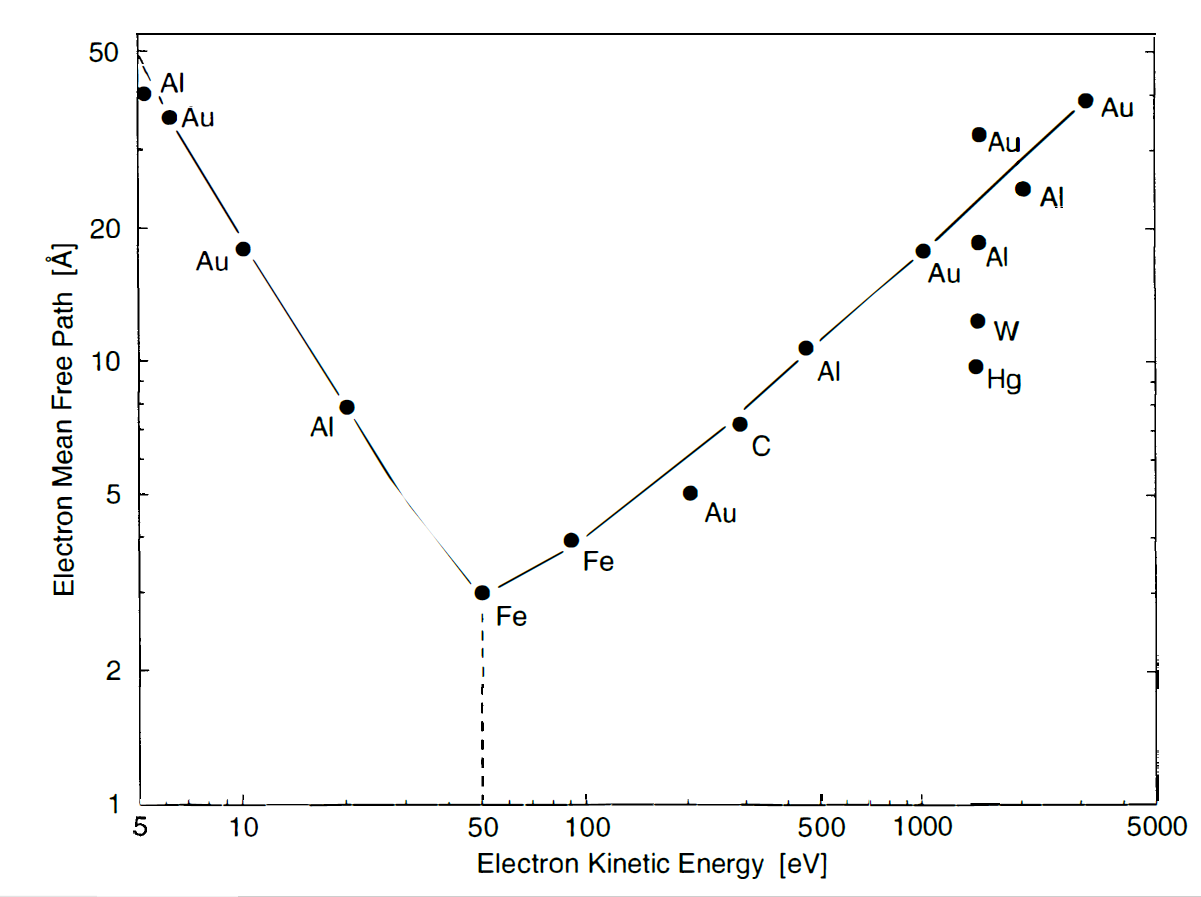
\includegraphics[width=0.7\textwidth]{./content/Weg.png}
        %     \caption{Die mittlere freie Weglänge für Elektronen in verschiedenen Materialien. Aus \textbf{Quelle}.}
        %     \label{fig:Weg}
        % \end{figure}
        Es ist zu erkennen, dass Elektronen mit einer kinetischen Energie im Bereich von \SIrange{30}{150}{\electronvolt} aus einer Tiefe von nicht mehr als \SI{5}{\angstrom} kommen.
        Werden also Elektronen als Sonden verwendet und ihre kinetische Energie angepasst, so kann davon ausgegagngen werden, dass sie nur aus Oberflächen nahen Bereichen kommen.

        Um Elektronen von der Probe kommend zu erhalten gibt es zwei Möglichkeiten.
        Zunächst kann man die Probe mit Elektronen im entsprechenden Energiebereich beschießen, die zurückkommenden Elektronen mit identischer kinetischen Energie können also nur aus oberflächen Nahemn bereichen kommen.
        Die zweite Möglichkeit ist es freie Elektronen in der Probe zu erzeugen, die dann aus der Oberfläche austreten und detektiert werden können.
        Die erste Möglichkeit wird bei der Beugung niederenergetischer Elektronen verwendet und die zweite bei der Photoelektronenspektroskopie.


    \section{Beugung niederenergetischer Elektronen} \label{sec:LEED}
        \begin{figure}
            \centering
            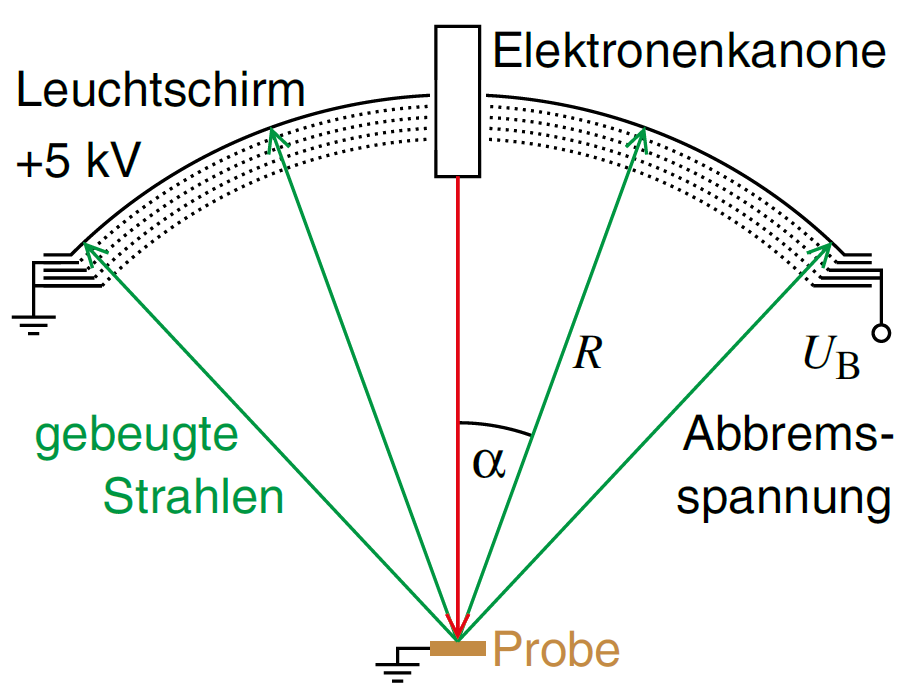
\includegraphics[width=0.5\textwidth]{./content/LEED.PNG}
            \caption{Innerer Aufbau der Apperatur zur Beugung niederenergetischer Elektronen. Aus \cite{Fauster}.}
            \label{fig:LEED}
        \end{figure}
        Um sich die geometrische Oberflächenbeschaffenheit genau anzusehen wir die Beugung niederenergetischer Elektronen (\textit{Low energy electron diffraction}, LEED) eingestezt.
        Hierbei werden Elektronen mit einer kinetischen Energie im Bereich der Oberflächensensitivität auf die Probe geschossen.
        Das entstehende Beugungsmuster ist charakteristisch für die Oberflächenbeschaffenheit und stellt die Oberfläche im reziproken Raum da.
        Der Aufbau mit seinen Optiken für die Beugung niederenergetischer Elektronen ist in Abbildung \ref{fig:LEED} abgebildet.
        
        Die Elektronen werden zunächst durch den Glühelektrischen Effekt erzeugt und durch einen Wehnelt-Zylinder gebündet.
        Diese beiden Komponenten bilden zusammen die Elektronenkanone.
        Anschließend werden Sie zur Probe hin beschleunigt.
        Da die Probe geerdet ist geschieht dies durch eine positive Vorspannung zwischen Probe und Elektronenkanone.
        Die gestreuten Elektronen bewegen sich in alle Richtungen unter dem Winkel $\alpha$ zum senkrecht auftreffenden Elektronenstrahl von der Probe weg.
        Damit die Flugbahn nicht durch elektrische Felder beeinflusst wird befindet sich das erste von der Probe aus gesehen Netz ebenfalls auf Erdpotential.
        Genau der Vorspannung entsprechend wird durch das dahinter liegende Netz  ein elektrisches Feld aufgebaut, gegen das die Elektronen anlaufen.
        So können nur elastisch gestreute Elektronen die weiteren Netze durchlaufen.
        Das nächste Gitter leigt wieder auf dem Erdpotential, damit das vom dahinter liegenden Gitter erzeugte Beschleunigungsfeld nicht durchgreift.
        Diese Beschleunigungsfeld wir durch eine hohe Spannung hervorgerufen und ist dafür notwendig, damit die Elektronen auf dem Leuchtschirm das Beugungsmuster erzeugen können.
        Mit Hilfe einer Kamera wird dieses Beugungsmuster erfasst.

        Die Entstehung des Beugungsmusters geschieht durch Interferenz Effekte, es ist also eine periodische Struktur von Nöten.
        Ebenso muss damit die Wellenlänge der Elektronen im Größenbereich der Gitterkonstanten liegen.
        Folglich haben die Elektronen einer Energie zwischen \SIrange{50}{200}{\electronvolt} \textbf{Quelle}.
        Für elastisch gestreute Elektronen muss also für den Impuls gelten $\abs*{\vec{k}_\text{i}} = \abs*{\vec{k}_\text{f}}$.
        Folglich darf der Impulsübertrag $\increment \vec{k}_{||}$ nur einen reziproken Gittervektor $\vec{g}_\text{hk}$ betragen, dies ist die Lauebedingung.     
        Intensitäten der einzelnen Spots $I$ ergeben sich dabei aus dem Formfaktor $F$ und dem Gitterfaktor $G$ zu
        \begin{equation}
            I = \abs*{F^2}\abs*{G^2}.
            \label{eqn:LEED}
        \end{equation}
        Mathematisch kommt der Formfaktor aus der Position der Atome innerhalb der Einheitszelle, wohingegen der Gitterfaktor die Periodizität der Gitters wiederspiegelt.
        Der Gitterfaktor ist nur ungleich Null, wenn die Lauebedingungerfüllt ist.
        Jeder Spot kann einem Impulsübertrag mit den Indizes $hk$ zugeordnet werden. 
        Größere Abstände im Realraum werden im reziproken Raum kleiner abgebildet.

            \begin{itemize}
                \item Geometrische Struktur
                \item Mathematische Methoden
            \end{itemize}

    
    \section{Photoelektronenspektroskopie} \label{sec:PES}
        \begin{itemize}
            \item Bespielspektrum mit den Bereichen
            \item Auger
            \item XPS
            \item UPS
            \item Fermikante
            \item Energieauflösung (Analysator, Thermisch, Photonenquelle)
            \item Sekundärelektronen
            \item Satellieten
            \item k senkrecht wegen gebrochener Periodizität nicht erhalten, k parallel berechenbar
            \item fermis Goldene Regel
            \item Plane wave approximation Ei und Ef
            \item WKF Kontrast
            \item Polarisationsfaktor $I \propto \abs{\vec{A} \cdot \vec{k}}^2$ A ist der Vektor des einfallenden E-Feldes
        \end{itemize}
        Die Grundlage ist der Photoelektronenspektroskopie ist der Photoelektrische Effekt, der 1905 zum ersten Mal von Albert Einstein erklärt wurde \cite{Einstein}.
        Hierbei werden Elektronen durch ein einfallendes Photon angeregt, ist die Energie hoch genug, so treten diese aus der Probenoberfläche aus.
        In Formeln ergibt sich so die kinetische Energie der Elektronen, die die Probe verlassen zu 
        \begin{equation}
            E_{\text{Kin}} = h \nu - E_{\symup{B}} - \psi
            \label{eqn:Photoeffekt}
        \end{equation}
        mit der Bindungsenergie des Elektrons $E_{\symup{B}}$, der Energie des einfallenden Photons $h \nu$ und der Austrittsarbeit $\psi$.
        Die Austrittsarbeit ist der Energieunterschied zwischen der Fermienergie und der Vakuumenergie.
        % \begin{figure}
        %     \centering
        %     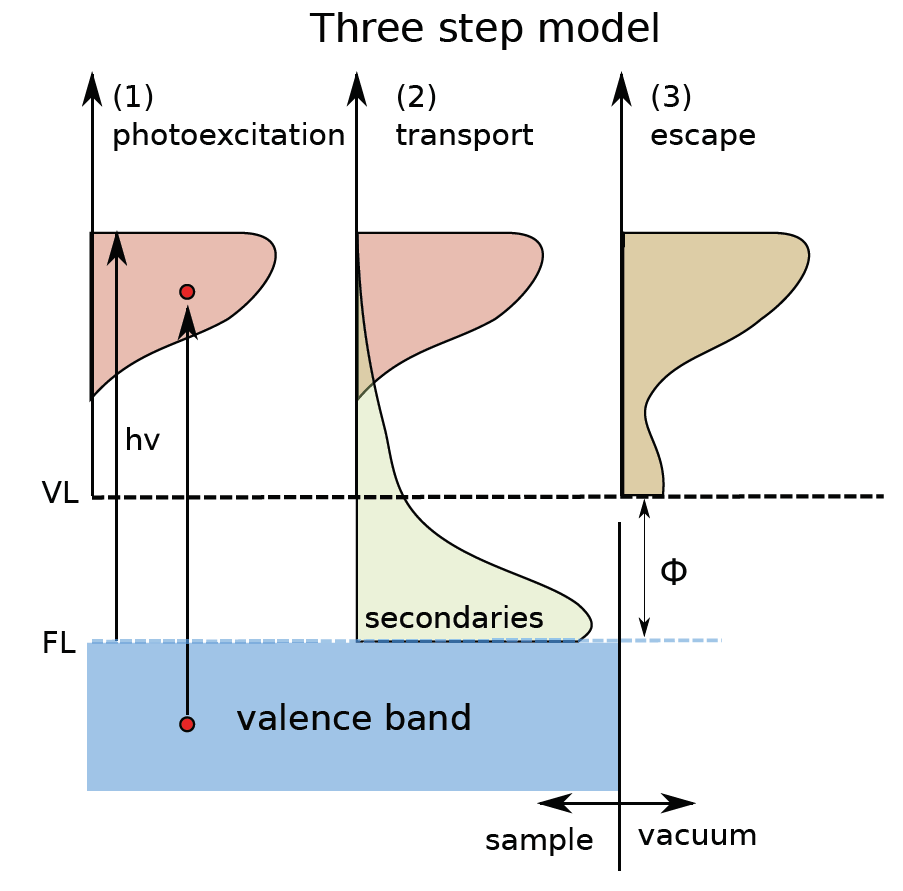
\includegraphics[width=0.7\textwidth]{./content/3Stufen.png}
        %     \caption{Schematische Darstellung des drei Stufen Models für den photoelektrischen Effekt. Aus \textbf{Quelle}.}
        %     \label{fig:3Stufen}
        % \end{figure}

        Dieser Prozess der Emittation eines Elektrons nach einfall eines Photons lässt sich in einem drei Stufen Model erklären.
        Das Model mit den Stufen ist in Abbildung \ref{fig:3Stufen} \textbf{BILD} schematisch zu sehen.
        Der erste Schritt ist die Absorption des Photons, wodurch das Elektron angeregt wird. 
        Dieses kann dann innerhalb des Festkörpers zur Probenoberfläche wandern.
        In diesem zweiten Schritt kommt auch die mittlere freie Weglänge der Elektroen zu tragen, weshalb die Methode oberflächensensitiv ist.
        Im dritten Schritt verlässt das Elektron die Oberfläche und wird auf Grund fehlender periodischer Strukturen gebeugt.

        Je nach Energie der verwendeten Photonen lässt sich in maßgeblich zwei Bereiche unterscheiden.
        Zum Einen in den Bereich der Röntgenstrahlung (\textit{X-Ray}), womit kernnahe Zustände untersucht werden.
        Zum Anderen den Bereich der Ultravioletten Strahlung, hier können Zustände nahe der Fermikante sichtbar gemacht werden.
        Die verschiedenen Energiebereich sind notwendig, damit die angeregten Elektronen eine kinetische Energie im oberflächensensitiven Bereich haben.
        Diese erste Methode wird XPS genannt, wohingegen die zweite Methode mit UPS abgekürzt wird.

        \subsection{Röntgenphotoelektronenspektroskopie}
            In den Energiebereich der Röntgenstrahlung fallen Photonen mit einer Energie von \SIrange{0}{0}{\electronvolt} \textbf{Quelle, Zahlen}.
            Diese Energien sind nur mit klassischen Röntgenquellen oder einem Synchrotron erreichbar.
            Mit dieser Methode lässt sich besonders gut die chemische Zusammensetzung untersuchen, da die kernnahen Zustände nur geringfügig beinflusst werden.

        \subsection{Ultraviolettphotoelektronenspektroskopie}
            Die Ultraviolette Strahlung besitzt einer Energie der Photonen im Bereich von \SIrange{0}{0}{\electronvolt} \textbf{Quelle, Zahlen}.
            Photonen in diesem Energiebereich können auch in Laboren mit Gasentladungslapen erzeugt werden, sind aber ebenfalls an Synchrotrons verfügbar.
            Diese Energien eignen sich besonders gut für Zustände nähe der Fermikante, also auch den Oberflächenzuständen.
            In diesen Bereich fallen auch die Energien die zur Molekülorbital Tomographie genutzt werden, welche in Kapitel \ref{sec:MOT} eingeführt wird.

        \subsection{Winkelaufgelöste Photoelektronenspektroskopie}
            Bisher wurde  auf den Austrittswinkel der Elektronen nicht genauer eingegangen, zumal bei XPS und UPS auch egeal ist unterwelchem Winkel die Elektronen die Probe verlassen.
            Diese Messungen werden meist auch in normaler Emission, also parallel zur Oberflächennormalen, vermessen.
            Über alle Austrittswinkel gemittelten Spektren werden auch als integrierte Spektren bezeichnet.
            % \begin{figure}
            %     \centering
            %     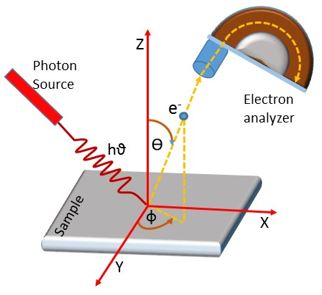
\includegraphics[width=0.7\textwidth]{./content/ARPES.png}
            %     \caption{Darstellung zur Anschaulichkeit von ARPES Messungen. Aus \textbf{Quelle}.}
            %     \label{fig:ARPES}
            % \end{figure}

            Die genaue Winkelverteilung der Elektronen wird bei der Winkelaufgelösten Photoelektronenspektroskopie genauer untersucht.
            Hierzu wird vom Analysator nur ein kleiner Winkelbreich akzeptiert und der Winkel zwischen Probe und Analysator stets varriert.
            Schematisch ist dies auch in Abbildung \ref{fig:ARPES} \textbf{BILD} dargstellt.
            Für jeden Messpunkt wird ein UPS Spektrum aufgezeichnet.


    \section{2D Photoelektronen Mikroskopie} \label{sec:2D-PES}
        \begin{enumerate}
            \item $E_\text{Pass}$
            \item Iris
            \item Integrierte Spektren (EDC, Electron density curve) spiegelt Zustandsdichte wieder
            \item kin. Energie zum Vakuum vermessen (Fermienergie plus Analysator Austrittsarbeit)
        \end{enumerate}
        Bei der 2D Photoelektronen Mikroskopie ist eine sehr viel versprechende Technik, die für immer mehr Aufsehen in den letzten Jahren gesorgt hat.
        Der größte Vorteil liegt wohl in der Kombination von spektroskopischen Methoden und mikroskopischen Methoden.
        Zuerst wurde dies 1933 durch E. Brüche entdeckt, der eine Zinkplatte mit Hilfe von Photoelektronen und einer magnetischen Linse auf einem Leuchtschirm abbildete \cite{bruche_elektronenmikroskopische_1933}.
        Sie nutzt die Prinzipien der Energie- und Impulserhaltung.

        \begin{figure}
            \centering
            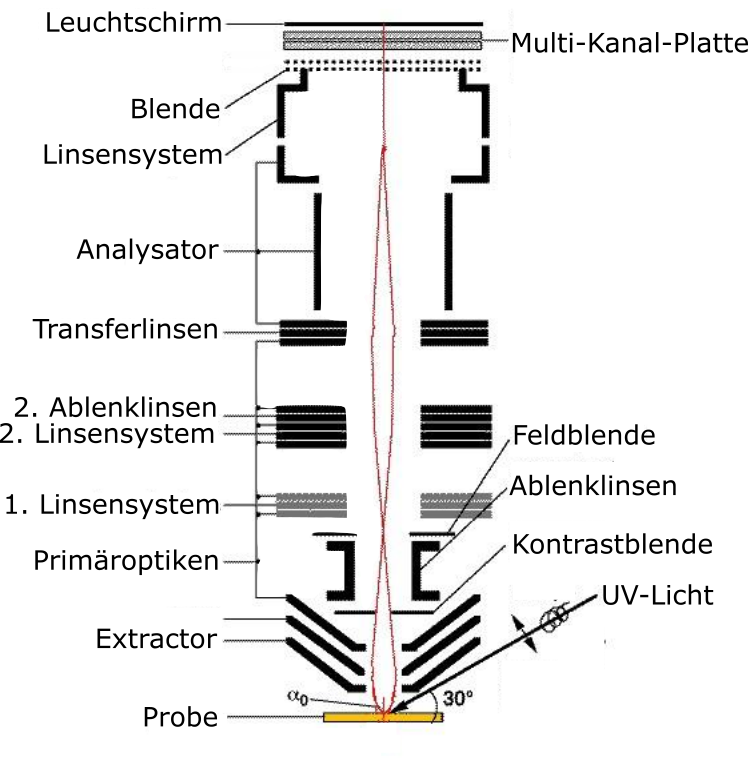
\includegraphics[width=0.7\textwidth]{./content/PEEM_schemaneu.png}
            \caption{Vereinfachter Aufbau eines 2D Photoelektronen Mikroskop. Vorlage aus \cite{KUCH}, modifiziert.}
            \label{fig:MM}
        \end{figure}
        Ein exemplarischer Aufbau ist in Abbildung \ref{fig:MM} zu sehen.
        Die durch die Photonen angeregten Elektronen werden durch ein starkes elektrisches Feld von einigen \si{\kilo\volt} von der Probe zum Analysator hin beschleunigt.
        Das Extractorfeld kann bis auf \SI{29}{\kilo\volt} erhöht werden, wird standardmäßig auf \SI{10}{\kilo\volt} festgesetzt.
        Durch diese große Spannung zwischen Probe und Extraktor ist es möglich ein ein großen Sichtbereich im Impulsraum abzudecken.
        Dies ist nötig, da durch den streifenden Einfall der Photonen und der Abberation der elektrostatischen Linsen nur einen kleinen Akzeptanzwinkel zur Verfügung stehen würde. \textbf{QUELLE}
        Wichtig bei der Kathoden Linse ist, dass das Feld zwischen Probe und Linse sehr homogen ist, damit der Austrittswinkel erhalten bleibt, dies hat zur Folge, dass die Probe auch eine möglichst ebene Oberfläche aufweisen muss.
        Anschließend werden die Elektronen durch elektrostatische Linsen fokusiert und durch die einzelnen Blenden geleitet.
        Sie sind so konzipiert, dass die Bildebene und die hintere Brennebene immer an der selben Position, der Blenden bleiben.
        Je nach dem an welcher Stelle eine Blende eingesetzt wird ergibt sich ein Bild im Realraum oder im Impulsraum.
        Damit der Spot auch immer im Zentrum der Blenden liegt gibt es im Linsensystem noch elektrostatische Verschiebungslinsen, welche den Strahl ablenken.
        Nach den Blenden folgt ein weiters Linsensystem aus elektrostatischen Linsen, welche das Bild auf den Ausgang des Linsensystems fokussieren.
        Hier befinden sich zwei magnetische Verschiebungslinsen um Drift zu korrigieren.
        Im Anschluss gehen die Elektronen in ein Transferlinsensystem über, welches dafür sorgt, dass ein einszueins Abbild auf die Eingagnsblende das Analysators trifft.
        Die Eingagnsblende kann in ihrer Größe varriert werden, sodass nur ein Teil der Elektronen in den Analysator eintreten.
        Je kleiner die Blende gewählt wird, desto besser ist die Energieauflösung aber so kleiner die Gesamtintensität.
        Als Energiealysator kommt ein hemisphärischer Analysator zum Einsatz, für gepulste Photonenquellen würde sich auch ein \textit{Time of flight - TOF} (Flugzeit) Analysator eignen.
        Bei dem hemisphärischer Analysator werden die Elektronen zwischen zwei Halbkugeln durch ein statisches elektrisch Feld auf eine Kreisbahn gezwungne.
        Dabei ist das Feld so gewählt, dass nur die mit der richtigen kinetischen Energie eintretenden Elektronen auch auf die Austrittsblende abgebildet werden.
        Bei einem TOF Analysators wird die kinetische Energie aus der Flugzeit der Elektronen bestimmt, weswegen es nur für gepulste Photonenquellen möglich ist.
        Nach dem Detektor gibt es eine weiter Linseneinheit, welche zusammen mit einer Blende das gewünschte energieaufgelöst Bild auswählt und es auf die Detektorgröße aufweitet.
        Anschließend durchlaufen die Elektronen eine Mikrokanalplate (eine Art Elektronenvervielfacher) und prallen auf den Phosphorschirm, der an den entsprechenden Stellen aufleuchtet.
        Durch die Kamera wird diese Leuchten regestriert und das räumliche oder rekrusives Bild kann rekostruiert werden \cite{SPECS-MM}.
        Bei dem Detektor handelt es sich um eine CMOS Kamera die das Bild der auf den Leuchtschirm auftreffenden Elektronen aufnimmt.
        Der Vorteil der CMOS (\textit{Complemantary metal-oxid-semiconductor}) Kamera Technik gegnüber der klassischen CCD (\textit{Charge Coupled Device}) Kamera Technik ist, dass erlaubt es wahre Pulszählraten zu erfassen 
        Dabei wird ein einzelnes Bild in nur wenigen Millisekunden erfasst, dies ist durch die Kombination von Kamera und Grafigprozessor möglich.
        Die CCD Detektoren sind ein Standard bei ARPES Messungen, sie integrieren die analoge Photonenintensitäten oder einzelne Lichtblize werden aufgezeichnet.
        Einer der Nachteile ist die geringe Abtastrate auf Grund der hohen Erholungszeit\cite{CMOS}.

        Es gibt zwei verschiedene Betribsmodi welche ferner erläutert werden.
        \begin{SCfigure}
            \centering
            \caption{Die verschiedenen Konfiguration der Blenden um zwischen Realraum Bild und Impulsraum Bild umzuschalten. Aus \cite{Focus}.}
            \label{fig:real_k}
            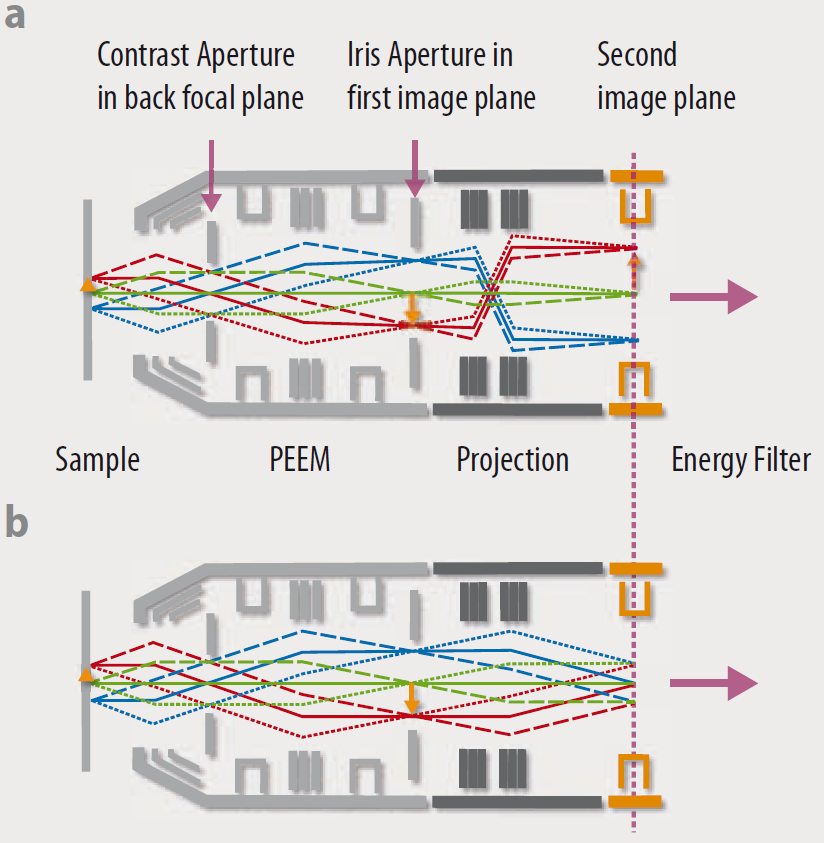
\includegraphics[width=0.7\textwidth]{./content/Real_k.PNG}
        \end{SCfigure}
        Für den Impulsraum ist dies in Abbildung \ref{fig:real_k}\,a und für den Realraum in Abbildung \ref{fig:real_k}\,b dargestellt.
        Vorteil der Umschaltung zwischen den Modis ist, dass auf sehr kleinen Bereichen die im Realraum bestimmt wurden dann auch Messungen im reziproken Raum durchgeführt werden können.


        \subsection{Impulsraum Aufnahmen}
            Um ein Bild im Impulsraum aufzunehmen wird die Blende im der Bildebene eingefahren, die so genannte Feldblende (\textit{field aperture}).
            Durch die Blende wird ein Ausschnitt auf der Probe ausgwählt, von der die emittierten Elektronen erfasst werden.
            Bei einem Blendendurchmesser von \SI{20}{\micro\meter} und der Standard-Vergrößerung von \num{5} ist der ausgewählt Bereich etwa \SI{4}{\micro\meter} groß.
            Bei der Aufnahme im Impulsraum wird bei der gesamten Abbildungsoptik der Austrittswinkel erhalten.
            So wird auf die Eintrittsblende des Analysators das Beugungsbild abgebildet.
            Das verwendete Mikroskop kann einen Austrittswinkel von biszu $\pm\SI{90}{\degree}$ erfassen für eine Energie kleiner als \SI{50}{\electronvolt} \cite[21]{SPECS-MM}.
            Für größere kinetische Energien wird das Sichtfeld auf $\pm\SI{3.6}{\angstrom}$ beschränkt.
            Dabei spielt es keine Rolle wo auf der Probe die Elektronen emittiert werden.

            Dies wird auch Impuls Mikroskopie (\textit{Momentum Microscopy}) genannt.
            Bei der Impuls Mikroskopie ist die zeitgleich Erfassung des polaren und azimuntalen Austrittswinkel von großer Bedeutung. 
            So entsteht durch die zusätzlich Sortierung der Elektronen nach ihrer kinetsichen Energie ein dreidimensionaler Datensatz.

        \subsection{Realraum Aufnahmen}
            Es ist ferner möglich Bilder im Realraum aufzunehmen.
            Dies geschieht durch Einsetzen einer Blende in dem hinteren Brennpunkt, die Kontrastblende (\textit{contrast aperture}).
            Dabei können sehr kleine Spots von \SIrange{50}{200}{\micro\meter} ausgewählt werden.
            Um den Kontrast im Bild zu erhöhen werden nur Elektronen mit einem bestimmten Austrittswinkel für die Erstellung des Bildes erfasst.
            Mit Hilfe der Kontrastblenden kann dann eine Auflößung von einigen \si{\nano\meter} erreicht werden \textbf{QUELLE}. 
            Auf dem Eintrittsspalt des Energyanalysators wird dann das Bild der Oberfläche projeziert.
            Das Bild wird bei festen Energiefilter-Einstellungen aufgenommen.

            Der Modi wird auch als PEEM (\textit{Photon emitted electron microscopy}) bezeichnet.

           
        
        \subsection{Erweiterungen}
            Als erweiterung der 2D Photoelektronen Mikroskopie sind auch zeitaufeglöste Messungen möglich.
            Hierbei erfolgt die Anregung mit zwei zeitlich versetzten Pulsen. 
            Dabei regt der erste Puls die Elektronen in einen höheren Zustand an und der zweite Puls löst diese dann aus.
            So ist es auch möglich zuvor unbesetzte Zustände (zwei Photonenemission) zu untersuchen.
            Wird der zeitliche Versatz zwischen den beiden Pulsen varriert so ist auch die Lebensdauer der Zustände abschätzbar.

            Mögliche Erweiterung wäre auch die Elektronen nach der Energieselection auch noch nach ihrem Spin zu sortieren.
            So lassen sich dann auch die magnetischen Eigenschaften genauer veranschaulichen.
        

    \section{Molekül Orbital Tomographie} \label{sec:MOT}
        Die Molekül Orbital Tomographie vereinigt nun die Vorteile der Impuls Mikroskopes mit der Theorie der Dichtefunktionaltheorie (DFT) um Molekülorbitale zu identifizieren.
        Aus der Theorie können die Orbitale der Moleküle in der Gasphase im Realraum berechnet werden \cite{database}.
        Werden diese dann Fourier transformiert, so erhält man die Aufenthaltswahrscheinlichkeiten der Elektronen abhängig von ihrem Impuls.
        Nun kann man die Moleküle bei einer bestimmten kinetischen Energie schneiden und erhält so ein zweidimensionales Bild \cite{brandstetter_kmappy_2021}.
        ferner kann auch die Wechselwirkungswahrscheinlichtkeit mit der verwendeten Photonenenergie berücksichtigt werden.
        Aus Messungen im Impulsraum kann dann durch einen Vergleich die Molekülorbitale zugeordnet werden.
        Dies ist nur möglich, wenn sich die Moleküle ordnen wie z.B. auf metalischen Oberflächen.

    \section{Versuchsaufbau}
        \begin{figure}
            \centering
            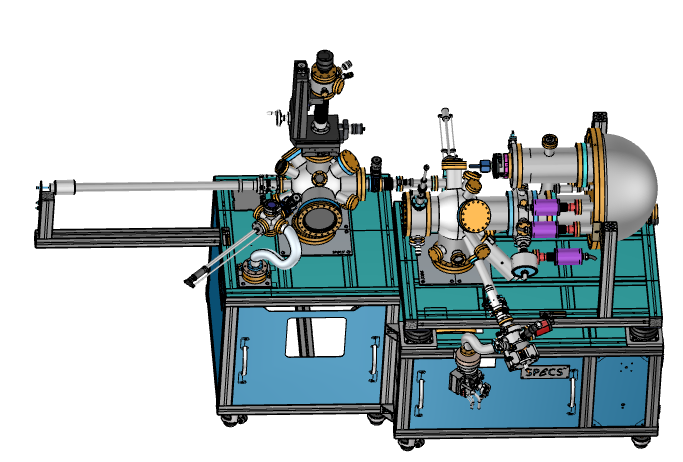
\includegraphics[width=0.7\textwidth]{./content/MM.png}
            \caption{Der für die durchgeführten Experimente verwendete Aufbau.}
            \label{fig:aufbau}
        \end{figure}
        Um die in dieser Arbeit untersuchten Proben zu präperieren und zu untersuchen wird der Versuchsaufbau in Abbildung \ref{fig:aufbau} verwendet.
        Dieser besteht aus einer Präperationskammer (links im Bild) und dem 2D Photoelektronen Mikroskop KREIOS 150MM von SPECS (rechts im Bild).

        Für die Reinigung der Probe steht eine Ionenquelle zur Verfügung, um die Probe mittels ioneninduzierter Zerstäubung zu reinigen.
        Auf dem Manipulator, mit dem die Probe im Ultrahochvakuum verfahren werden kann, ist eine Elektronenstoßheizung montiert um die Probe aufzuheizen.
        Die Präperationskammer ist mit einer LEED-Optik ausgestattet um die Oberflächenbeschaffenheit zu kontrollieren.
        Ferner befindet sich noch ein Leckventil für Sauerstoff sowie Molekül- und Metallaufdampfer an der Kammer.
        
        Vor der Extraktorlinse des 2D Photoelektronen Mikroskopes befindet sich eine 6-Achsen-Piezostage (Hexapod) mit der die Probe in Position gebracht und ausgerichtet werden kann.
        Messungen erfordern eine exakte Ausrichtung der Oberflächennormalen parallel zur Linsenachse und ferner einen Abstand von \SI{4}{\milli\meter} zum Extraktor.
        Mit dieser Positioniereinheit kann die Probe auch auf unter \SI{10}{\kelvin} abgekühlt werden.
        Als Photonenquelle steht eine Helium-Gasentladungslampe bereit, welche größtenteils Photonen der He-I-Linie emittiert.